\chapter{Data sources and data formats}
Signals for OSA come from many different sensor data sources. Moreover, the quality of these signals is diverse. Signals that come from clinical grade sensors are used in the medical domain, while signals that come from consumer electronic sensors are often used for fitness trackers, research, etc. In other words, consumer electronic sensors are not allowed in medicine, because they have not been approved yet. Therefore, a hypothesis is made that the signals from clinical sensors have better quality than the consumer electronic sensors. This chapter presents two corresponding sensor data sources for these two types of sensors. Consumer electronic signals come from BITalino sensors while clinic grade signals are stored in the Physionet database and captured with clinical grade sensors. In addition, different sensor data sources provide different formats to obtain and store the signals. Therefore, this chapter also presents a description of data formatting for each of the sensor data sources. In Section 3.1, an overview of data sources is presented. Section 3.2 presents different methods to format data signals. Standard formats, which are the European Data Format (EDF)\cite{EDF1} and the European Data Format plus (EDF+) are presented in Section 3.2. Section 3.3 presents two data acquisition tools that can be used to obtain biosignals from sensor sources.
\section{Data sources}
    In general, the quality of data has a huge influence to the data analysis process. Better analysis results are often derived from a higher quality data source. Therefore, choosing a good data source is vital for analyses. Misleading results are caused by various reasons, and a low quality data source is one of the major causes. However, a good source often comes with a very expensive price. In medicine, for obtaining biosignals has to follow strict requirements, and often use expensive clinical grade sensors to harvest these signals. The clinical data sensors provide high quality signals which can create a high quality dataset. After all, it is much more expensive to buy and maintain a clinical sensor system than a consumer electronic sensor system. For example, a NOX-T3 from nox-medical costs 55000kr plus value added tax\cite{Thomas} while a BITalino costs about 1000kr. The consumer electronic sensors often come with reasonable or even low price, because the quality of signals have not been approved, or maybe they are not good as the signals from the clinical sensors. However, there are many publications on using the consumer electronic sensors each year (for the BITalino 14 publications in 2015 and 7 publications in 2016\cite{BITalinoPubs}). Hence, an assumption is made that the quality of signals which is provided by the consumer electronic sensors is good enough to do research, build commercial applications etc. Nevertheless, the quality of biosignals and the support from consumer electronic sensors are promised to be improved in the future, because many leading companies constantly searching and integrated health care into their products, for example: Google Fit, Apple Health and Fitness, Microsoft band and Microsoft health, Xiaomi band, etc. This section presents an overview of BITalino which is one of the consumer electronic sensor groups for biosignals that has been used widely in many projects, products and researches, and Physionet database as clinical grade sensors source.
    \subsection{Data from BITalino sensors}
        BITalino is one of the reasonable priced sensor hardware platform which is easy to use and configure. BITalino is marked as DIY which means "do it yourself", therefore the goal of it is to use it for building an all-in-one platform such that every one can easily create their own biomedical devices. It is easy to configure, because BITalino is a plug-and-play device. The pre-conditioned analog outputs are sent wirelessly via bluetooth. Moreover, there are dozen of free, open source and paid softwares that support the BITalino sensor kit. These softwares can run on various operating systems, for example Linux, OSX, Windows, Android etc. Nevertheless, BITalino is not a medical device or to be used in medical diagnosis as they mentioned in their disclaimer on the website \cite{BITalino}. It is for students, teachers, researchers, etc., who do not need to have any engineering electrical skills to use it.
        \subsubsection{BITalino Kit}
            BITalino has a wide rang of sensors. Those sensors have the capability to measure either bio-electrical or bio-mechanical signals. BITalino has three major components that together form a basic bio-harvesting device. The first component is the power management which provides and manages power for biosignals acquisition. The BITalino power component uses a 3.7V LiPo battery to power its analog and digital parts. The second component is the micro controller unit (MCU) which is designed for accurate and reliable real-time streaming. It can control up to 6 analog inputs, 1 output, 2 digital inputs and 2 digital outputs at up to 1kHz \cite{BITalino_MCU}. The third component is data transfer. Data transfer is either bluetooth (BT) or bluetooth low energy (BLE), and is a ready-to-use module. The rest of the components are organized as independent modules that can be attached to the main board on demand.
            
            BITalino provides three kits: BITalino (r)evolution board, BITalino (r)evolution freestyle and BITalino (r)evolution plugged.\footnote{The evolution version is discontinued. The next generation of the BITalino is revolution, it has almost 2x the blocks and up to 60\% smaller sensors.}\\
            \begin{figure}[ht]
                \centering
                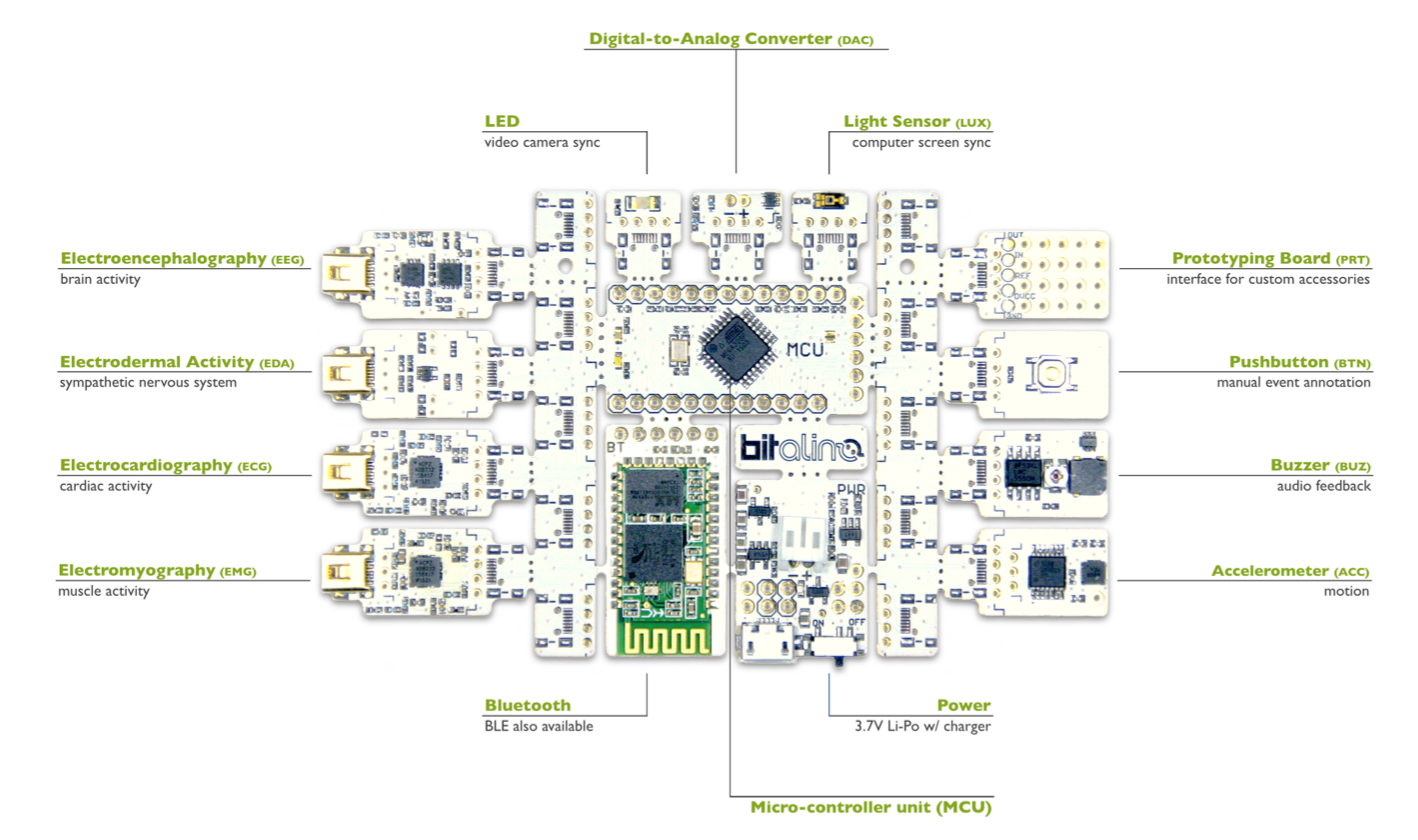
\includegraphics[width=1.0\textwidth]{Figures/BITalino_board.png}
                \caption{BITalino (r)evolution Board with Bluetooth connectivity \cite{BITalino_board}}
                \label{fig:Figures/BITalino_board}
            \end{figure}\\
            Figure 3.1 illustrates the BITalino (r)evolution board\cite{BITalino_board}. The size of the board is 100x65x6mm, and it is powered by a 3.7V recharge battery. The board consists of analog ports (4in - 10bit, 2in - 6bit, 1in - battery, 1out - 8bit) and digital ports (2in - 1bit, 2out - 1bit). In addition, it has either BT or BLE which have a range about 10m. There are seven sensors which are integrated on the board. They are electromyography (EMG), electrocardiography (ECG), electro-dermal activity (EDA), electroencephalography (EEG), accelerometer (ACC), light (LUX) and pushbutton (BTN). The board kit is designed as all-in-one device. The board connects all the necessary components which are the power management, MCU, BT and sensors into one board which is ready to use. This kit is made for biosignal exploration and lab activities. In conjunction with the OpenSignals software, it provides real-time biosignal data visualization.\\
            \begin{figure}[ht]
                \centering
                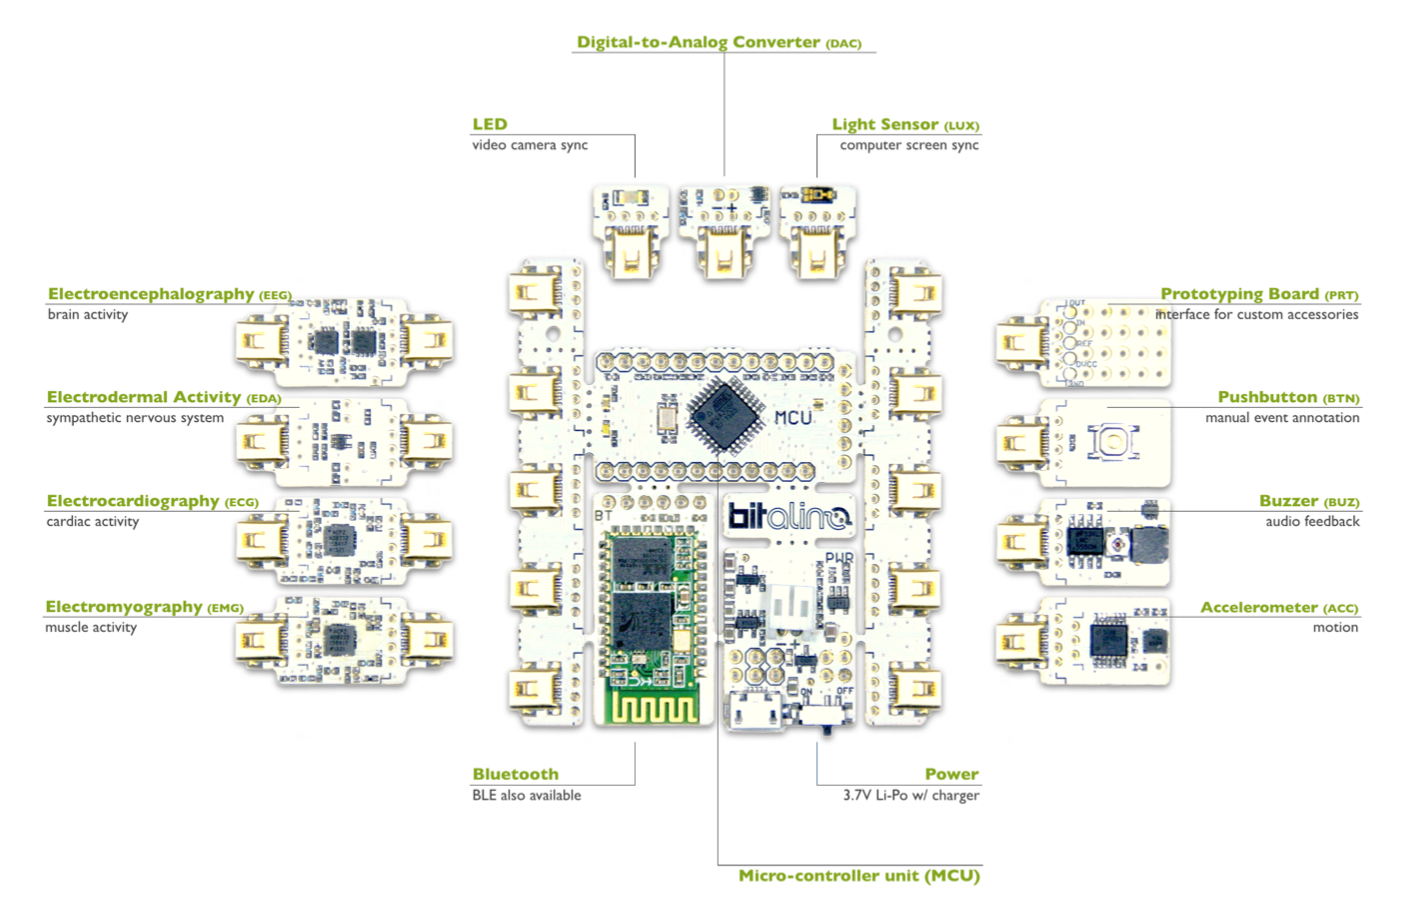
\includegraphics[width=1.0\textwidth]{Figures/BITalino_plugged.png}
                \caption{BITalino (r)evolution Plugged with Bluetooth connectivity \cite{BITalino_plugged}}
                \label{fig:Figures/BITalino_plugged}
            \end{figure}\\
            Figure 3.2 illustrates the BITalino (r)evolution plugged\cite{BITalino_plugged}. It is similar to the board kit, however the main board contains only three major components which are power management, MCU and BT. The main board also provides analog and digital ports to the inputs and outputs. The sensors do not integrate on the main board, they are separated from the board and connected as plug and play on demand. Therefore, the plugged kit provides maximum flexible configuration.\\
            \begin{figure}[ht]
                \centering
                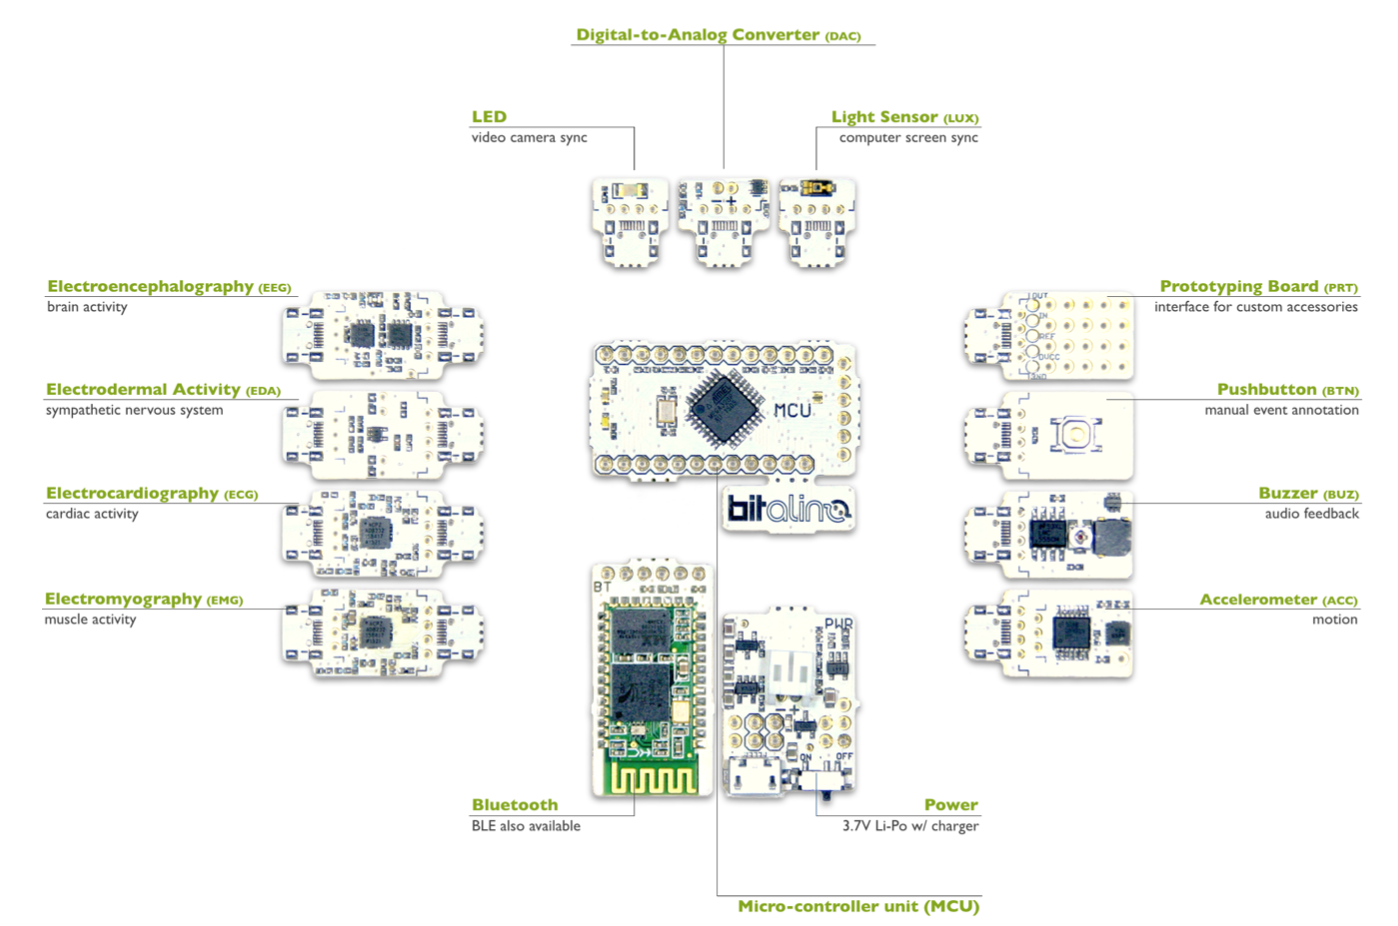
\includegraphics[width=1.0\textwidth]{Figures/BITalino_Freestyle.png}
                \caption{BITalino (r)evolution Freestyle with Bluetooth connectivity \cite{BITalino_Freestyle}}
                \label{fig:Figures/BITalino_Freestyle}
            \end{figure}\\
            Figure 3.3 illustrates the BITalino (r)evolution freestyle\cite{BITalino_Freestyle}. As the name of the kit, it provides maximum configuration. Hence, the users can maximize their imagination in building wearable biosignal acquisition devices. Each component is separated in a individual module, even the power management, MCU and BT are not on the same board.\\
        \subsubsection{BITalino sensors}
            This section briefly describes the sensors, i.e., EMG, ECG, EDA, EEG, ACC, LUX, BTN, PZT, that are provided by BITalino.\\
            The ACC sensor translates the motion into numerical values. BITalino provides 3-axis sensing for detecting tilt, monitoring activity, and measuring vibration. The sensor is limited in acquiring data from bio-mechanical and kinematic events. The sensor can be used in detecting posture, fall or shock, estimating rang of motion, step counting etc. Although it has 3 axis sensing, only the Z-axis is connected by default. It is because three analog outputs can be accessed separately, and the user can easily connect the X-axis and the Y-axis as their project demands.\\
            The ECG sensor translates the bio-electrical signals, which are low amplitude and generated by a set of cells in the heart, into numerical values. The ECG sensor from BITalino can obtain data not only at the chest, but also at the hand palms. Furthermore, the sensor works with pre-gelled electrodes as good as most types of the dry onces. According to ECG sensor data sheet, the sensor provides bipolar differential measurement with pre-conditioned analog output, and has a small form factor, and high signal-to-noise ratio. Therefore, it is widely used in heart rate and heart variability applications.\\
            The EDA sensor translates the resistance of the skin into numerical values. The human body secretes sweat not only when the body needs to regulate temperature, but also when the sympathetic nervous system activity is affected, for example when relaxing or arousing. The BITalino EDA sensor provides pre-conditioned analog output with high signal-to-noise ratio from measuring skin resistance. This signal is widely used in many applications such as lie detector, relaxation etc. and in this thesis it is used for detecting arousal and emotional cartography.\\
            The EMG sensor translates the bio-electrical signals which are sent from motor control neurons in the brain to the muscle fibers. A BITalino EMG sensor works with both dry and pre-gelled electrodes. This sensor has a wide range of applications such as muscle reflex studies, nerve conduction measurement, human-computer interaction etc.\\
            The LUX sensor translates the intensity of light into a digital signal. The BITalino LUX sensor can be adapted to human eye responsiveness.\\
            The push button is useful for taking the annotation of meaningful events which occur during the observation.\\
            BITilano TMP sensor translates the temperature of a body or the environment into digital values which range from -40C to +125C. The accuracy of the sensor varies from -2C to +2C, and the linearity is 0.5. It is small (about 12x27mm) and has low power consumption (about 0.05mA) which are good properties for building wearable devices.\\
            PZT sensor translates the displacement variations induced when inhaling or exhaling into numerical values. BITalino PZT sensor consists of a adjustable chest strap, RJ22 connector and a sensor which is secured in the chest strap. A BITalino PZT sensor is a good option for respiratory analysis.
        \subsubsection{Logical sensors}
            A sensor network consists of dozens of sensor. Sometimes some of them need to be taken down for maintenance, or the network needs to integrate additional sensors to form a bigger network. A methodology has been introduced by C.Hansen et.al\cite{LOGICALSENSOR_1} in November 1983 to deal with the problem, which is a logical sensor. The overall goal of logical sensors is to aid in the coherent synthesis of efficient and reliable sensor systems. There are two problems regarding to sensor systems\cite{LOGICALSENSOR_0}. The first problem is how to build an efficient and coherent method for the information provided by various kinds of sensors. The second problem is how to maintain and develop the system for that it can be incorporated with additional sensing devices. Sensor data abstraction is introduced for solving these problems. Data abstraction techniques are used to analyze and create patterns (logical sensors) from sensor data\cite{SensorDataAbstract}. The patterns are considered the interfaces for sensor systems which make the systems easily to be reconfigured in the future. Furthermore, the patterns together with the sensor semantic descriptions help to minimize the size of the data which is sent from the sensor nodes to the gateways or high level processing components. There are many principle motivations for logical sensor specification. Three of them are emergence of multi-sensor systems (a coherent data acquisition and integration system is needed), benefits of data abstraction (an inherent hierarchical structuring of logical sensors further aids system is needed) and availability of smart sensors (substitution of hardware for software and vice versa)\cite{LOGICALSENSOR_3}.
    \subsection{Physionet sensor databases}
        As mentioned earlier, the quality of data plays a very important role in choosing data sets. Especially for biosignals, the data must be from the trustworthy sources. Therefore, Physionet sensor databases are chosen as trustworthy clinical grade sources. Physionet is inaugurated by the researchers at Boston's Beth Israel Deaconess Medical Center, Boston University, McGrill University and MIT\cite{PhysioNet_Intro}. To date it is supported by the National Institute of General Medical Sciences and the National Institute of Biomedical Imaging and Bioengineering. Physionet has three interdependent components which are PhysioNet, PhysioBank and PhysioToolkit. The first component is PhysioNet which is used for exchanging and disseminating the biomedical signals and the software used to analyze those signals. PhysioNet also offers training opportunities\cite{PhysioNet_Training} that consist of tutorials on a variety of topics, special designed data sets for classroom activities and annual open challenges. PhysioBank is the second component which contains biosignal databases from various kind of diseases. PhysioBank unceasingly grows in both size and scope, to date even signals from vivo and vitro experiments are accepted \cite{PhysioNet_Contributing}. The last component is PhysioToolkit which provides tools for analyzing the biomedical signals. There are four databases in Physionet that can be used for analyzing OSA. They are apnea-ECG database, St. Vincent's University Hospital database, MIT-BIH polysomnographic database and SHHS polysomnography database.\\
        \textbf{Apnea-ECG database\cite{Apnea_ecg_db}: }\\
        This database has been created for Computers in Cardiology Challenge 2000 (CinC Challenge 2000). It was provided by Dr. Thomas Penzel of Phillipps-University, Marburg, Germany\cite{CinC2000}. The data consist of 70 records that are equally divided into two data sets. One is a learning set, the other is a test set. Each record has a 100 Hz with 12-bit resolution ECG signal which is digitalized and lasts for slightly less than 7 hours to nearly 10 hours. In addition, the record also contains a set of apnea annotations. The apnea annotations are marked by physicians whether an apnea event happens or not, one annotation per minute. However, the apnea annotations are not available in the test set due to the challenge, but are made available after the contest. The annotations include age, gender, height, weight, apnea index, hypopnea index and apnea-hypopnea index. Eight records which are called a01 to a04, b01 and c01 to c06 have extra four additional signals\cite{Apnea_ecg} for chest and abdominal respiratory effort, oronasal airflow, oxygen saturation in which the oxygen saturation signal digitized at 1Hz while the rest digitalized at 20Hz. Those additional signals are used as learning material to study the relationships between the respiration and ECG signals.\\
        These records are harvested between 1993 and 1999 \cite{Apnea_ecg_db}. During 1998 to 1999, the ECGs were digitized at 200Hz. However, to synchronize with the ECGs which are taken during 1993 and 1995, the newer ECGs were decimated to 100Hz. Therefore all records in the data set have 100Hz ECG signal. The signals are from three groups of subjects: the apnea group, the "borderline apnea" group and the normal group. The mean age of these three groups is slightly different, the higher the mean age, the more severe the apnea. Furthermore, due to lack of episodes of pure central apnea or of Cheyne-Stokes respiration, obstructive and mixed apnea can not be distinguished in this data set, this is to say a hypopnea minute is the same as an apnea minute. Nevertheless, the Apnea-ECG database is a good source to use for studying and doing research on sleep apnea.\\
        \textbf{St. Vincent's University Hospital database: }\\
        St. Vincent's University Hospital Sleep Disorders Clinic has collected 25 full overnight polysomnograms records with three-channel Holter ECG. The clinical and demographic information were at first collected and assembled under the guidance of professor Walter McNicholas, Dr. Liam Doherty, Dr. Silke Ryan and Dr. John Garvey, then scored and annotated by Ms Patrica Boyle, finally anonymized and electronic ally archived by Eric Chua. Signals which are monitored and stored are EEG, left EOG, right EOG, submental EMG, ECG, oronasal airflow, ribcage movements, abdomen movements, oxygen saturation, snoring and body position. The EDF format is used to save the records. Monitored subjects are above 18 years old, and randomly selected from patients referred to the clinic for that no known diseases can interfere with the heart rate. As a result, there are 25 subjects selected, i.e., 21 males and four females with the age range from 28 to 68 years, and the measured AHI range from 1.7 to 90.9\cite{STVinceUniversity}.\\
        \textbf{The MIT-BIH polysomnographic database: }\\
        The MIT-BIH polysomnographic database contains 16 subjects with sleep apnea syndrome from 60 male subjects in the age range of 32 to 56 years and a weight range from 89kg to 152kg\cite{MIT_BIH_slpdb}. This database is made for researchers who want to investigate clinical physiology, for engineers who want to develop a new method to analyze the digitized polysomnography data, and for students who want to learn sleep physiology. These subjects were observed in Boston's Beth Israel Hospital Sleep Laboratory for evaluating and testing CPAP. The monitored signals under observation are ECG, BP, EEG, Resp, EOG, EMG, SV and SO2 which have a sampling rate of 250Hz with 12-bit resolution. The recording time for each subject lasted from two to seven hours. This database is one of the most trustworthy resources for investigating and learning.\\
        \textbf{The SHHS polysomnography database: }
        The Sleep Heart Health Study polysomnography database is used for determining the relationship between cardiovascular diseases and other consequences of sleep-disordered breathing. From 1995 to 1998, 6441 men and women with the mean age of 40 took part in the sleep-related breathing examination\cite{SHSH_SleepData}. The participants can stay at their home under extermination, and are monitored by trained technicians. The recoded signals include EEGs at 125Hz, EOGs at 50Hz, EMG at 125Hz, thoracic and abdominal movements at 10Hz, nasal-oral airflow at 10Hz, finger-tip pulse oximetry at 1Hz, ECG at 125Hz, heart rate at 1Hz, body position and ambient light. There is only one polysomnogram sample which is formated in the EDF form available in Physionet. However, more data can be downloaded freely via the National Sleep Research Resource website\cite{SHSH_NationalSleepData}. Since this database was made by a multi-center cohort study which are supported by the National Heart Lung \& Blood Institute, it is also considered one of the most trustworthy resources for investigating and learning.
\section{Data formats}
    When collecting signals, the selection of a structure for storing data is very important issue. The selected structure must provide fast accessing, support cross platform, extensibility, multi modality, querying etc. In other words, this selection depends on the experiences of expert groups in implementing projects, the quality and the performance of the final result. Therefore, each group has its own data format for its special tasks. After choosing the data format, a set of rules are provided such that the database can be used outside the group. The problems raise when the number of groups increases. Hence, a standardized data format for biosignals is very essential for that these bio-research groups and clinics can not only coordinate and share data in an efficient way, but they can also improve the quality of the software.\\
    \subsection{Physionet sensor database formats}
        Although the stored data in the previously described four databases are biosignals, the format for each database is different.\\
        \textbf{Apnea-ECG database: }\\
        Apnea annotations are stored in the .apn and .qrs files\cite{Apnea_ecg_annotation}. In the .apn files, a one-minute interval is used between annotations. A "A" annotation presents that apnea was in progress at the beginning of the fellowed minute while a "N" annotation shows that apnea was not in progress at the beginning of the fellowed minute. Rdann\footnote{Rdann is a program that reads and converts the binary annotations files into text, one annotation per line.} needs to be used for converting the binary annotations in these files into text for viewing. However, the .qrs files can be viewed by using sqrs125\footnote{sqrs125 is a program that locates QRS complexes in an ECG signal in the specified record.}. In the .qrs files, all observed heart beats are marked with "N" annotations, and QRS-like artifacts are marked with "\textbar" annotations\cite{Apnea_ecg_annotation}.\\
        \textbf{St. Vincent's University Hospital database: }\\
        Unlike the way Apnea-ECG database stores its annotations (encoded its annotations), St. Vincent's University Hospital database has the annotations in a text file, the *\_stage.txt and *\_respevt.txt files. Figure 3.4 presents two tables for annotations in these files:
        \begin{figure}[ht]
        \centering     %%% not \center
        \subfigure[Annotations for *\_stage.txt\cite{STVinceUniversity_ann}]{\label{fig:VUH_ANN_S}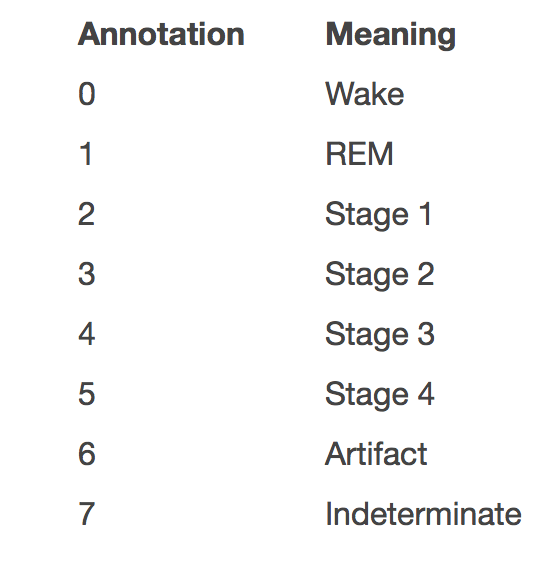
\includegraphics[width=50mm]{Figures/VUH_ANN.png}}
        \subfigure[Annotations for *\_respevt.txt\cite{STVinceUniversity_ann}]{\label{fig:VUH_ANN_R}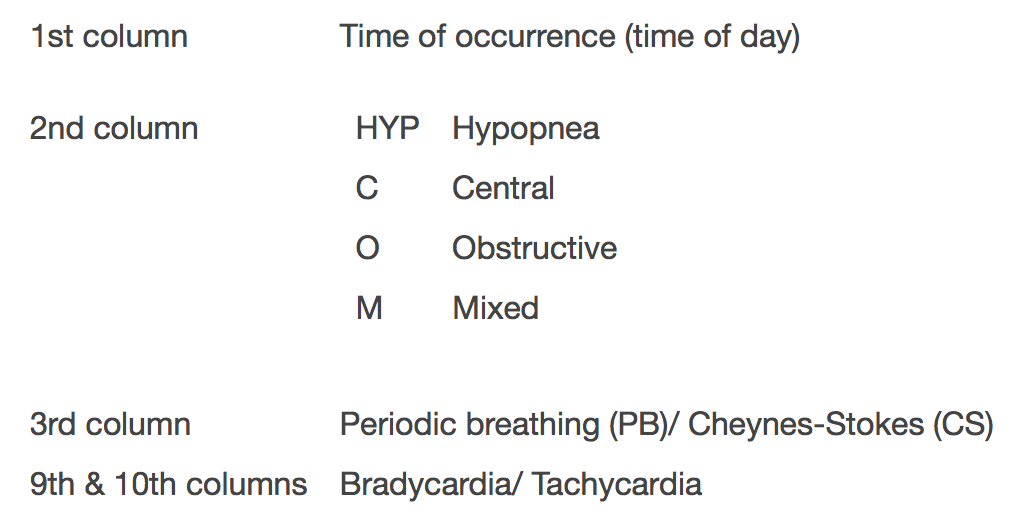
\includegraphics[width=90mm]{Figures/VUH_ANN_respevt.png}}
        \caption{Annotations for St. Vincent's University Hospital database}
        \end{figure}\\
        \textbf{MIT-BIH polysomnographic database: }\\
        Each record in this database has two annotations files, there are .ecg and .st files. The .ecg file contains the beat annotations in wave form while the .st file stores the sleep stage and apnea annotations. Therefore, the .ecg files can be read by following WFDB Programmer's Guide which is made by George B.Moody\cite{MIT_BIH_WFDB}. The .st files contain note-annotations which are sleep staging and apnea information.\\
        \textbf{SHHS polysomnography database: }
        The annotations of this database can be read by using PhysioBank ATM\cite{SHSH_Physiobank} which is free to use from Physionet. The PhysioBank ATM can export the annotations to many different data formats, for example CVS, EDF, Matlab etc. The .hypn contains annotations for sleep stage, the .arou files contains the information on arousal event type and duration, the .oart files contains annotations which present oxygen saturation (SaO2) and their duration, the .resp files contains the annotations for apnea event together with their duration and percent decrease in SaO2, minimum SaO2. The database has also .comp files that are compressed files. The .comp files contains all of the annotations that are stored in the .hypn, .arou, .resp, and .oart files.
    \subsection{EDF and EDF+ formats}
        In recent decades, many efforts to standardize the data format for biosignals have been done. One of them is the European Data Format (EDF). EDF is used for exchanging and storing multichannel biological and physical signals in a simple and flexible way. It was first introduced in 1987 at the Sleep Congress in Copenhagen and then contributed by all participating labs in August 1990\cite{EDF1}. The first publication of EDF was in 1992 in Electroencephalography and Clinical Neurophysiology 82, pages 391-393. The next version of EDF is EDF plus. It was published in 2003 and is compatible to the original EDF version. This is to say all existing EDF viewer programs can use EDF+. On the other hand, EDF+ can contain interrupted recordings as well as annotations, stimuli, and events. It has also fixed some problems that existed in EDF such as Y2K problem, comma vs dot, little-endian integers. Moreover, the EDF+ also supports UTF-8 format. The EDF+ is used in polysomnography, EEG, ECG, EMG and sleep scoring applications. Last but not least, EDF and EDF+ are free to use, and the users and developers can get supports from the EDF site via free downloads of files and software.
        \begin{figure}[ht]
            \centering
            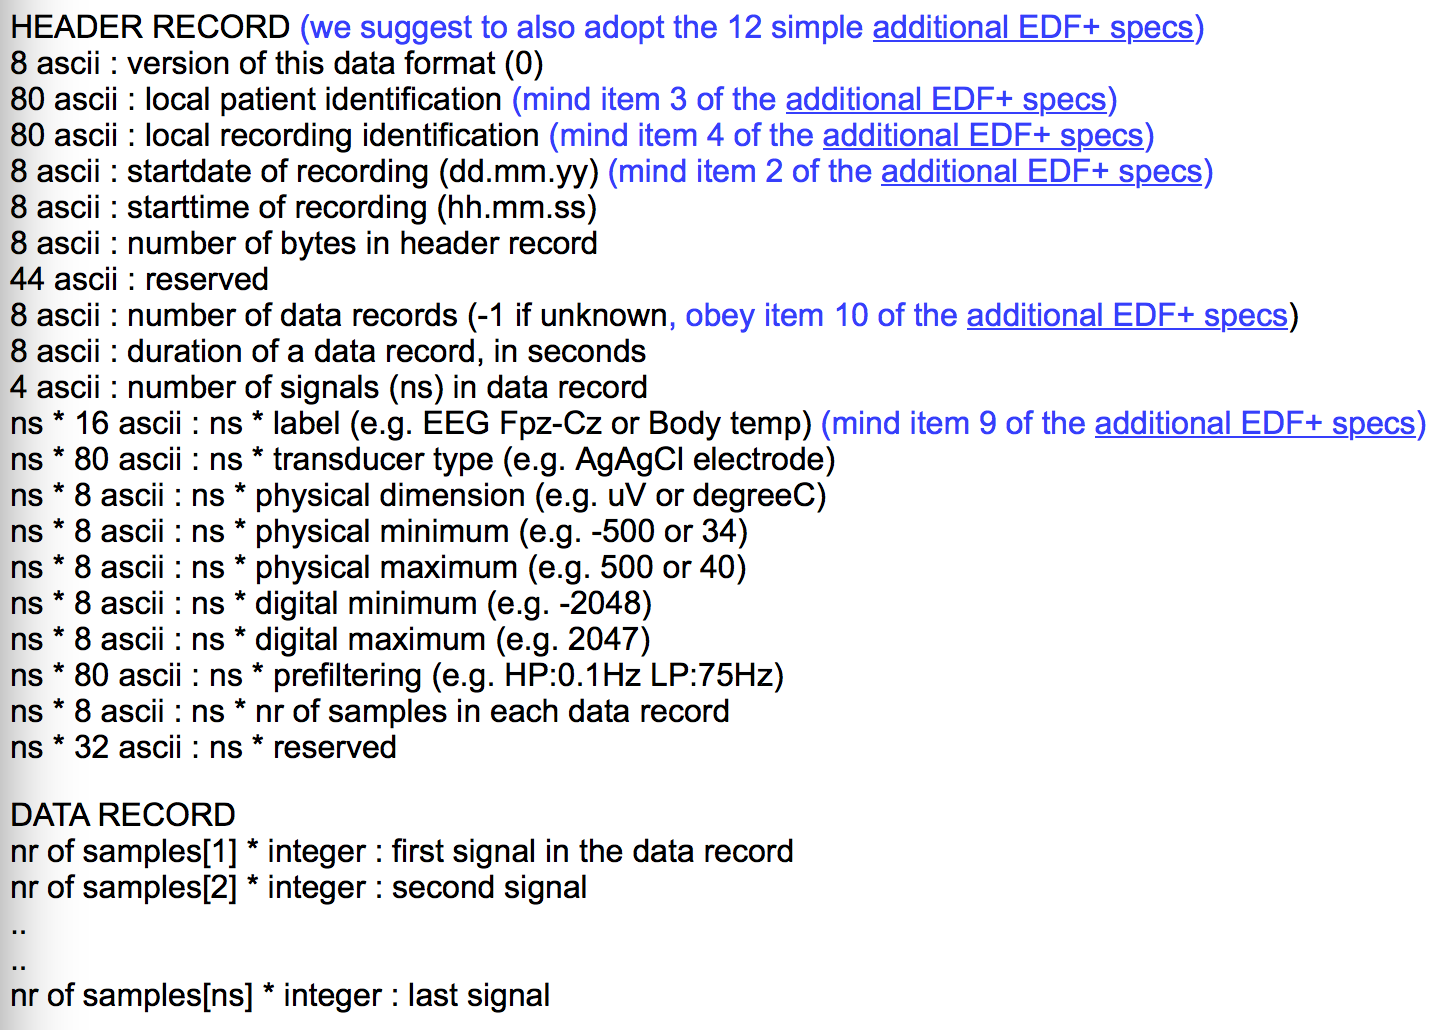
\includegraphics[width=1.0\textwidth]{Figures/EDFFILE.png}
            \caption{EDF and EDF+ file structure \cite{EDF2}}
            \label{fig:edf}
        \end{figure}\\
        Both EDF and EDF+ have the same structure of a data file. As Figure 3.5 presents, the data file consists of two parts which are the header record and the data records. The first 256 bytes of the header part contains the basic information for the record which are the version of the data format (8 ascii), the identifications of the local patient and the local recording (80+80 ascii), start date formated as dd.mm.yy (8 ascii), start time formated as hh.mm.ss (8 ascii), the size of the header record (8 ascii), reserved field (44 ascii), the number of data records followed by the header record (8 ascii), duration of a data record (8 ascii), and the number of signals in data record (4 ascii). The rest of the header record (after the first 256 bytes) contains the information for each field of the signals. Each signal has a label which is not longer than 16 bytes, and coded in ascii. After the label is the transducer type which has the length up to 80 bytes. After the transducer type field is the physical dimension with its maximum and minimum observable values (both physical and digital), each of them is coded in 8 ascii bytes. The following 80 bytes are used to store filters which were used for the signal. The next 8 bytes are used for the number of samples in each data record. The last 32 bytes are reserved.\\
        The data record part consists of a list of data records. Each data record has a list of samples for each signal. For each signal in the record, a sample for the signal is an integer. Hence, the number of bytes for each signal is the number of sample multiply with the size of integer.\\
        The differences between EDF and EDF+ are the information in the 44 bytes reserved field and additional specifications are added to EDF+. In the reserved field, when a record is EDF+ and continuous, it must start with EDF+C, and EDF+D if it is discrete. There are 12 additional specifications in EDF+ which are some rules for the header, date-time, local patient and local recording identification, digital maximum and minimum, separator for digital grouping, endian format, standard texts and polarity rules etc.\cite{EDFpluss}.\\
        The EDF+ data files are coded in a way that they can store both annotations and events. The EDF software can read EDF+ annotations as the physical sensor signals. Because the annotations are treated as signal, the results that are presented in the EDF viewers are strange.\\
        Beside containing ordinary signals, EDF+ can contain annotations signals. The annotations signal is defined by giving it the label "EDF Annotations". Then instead of storing ordinary signal samples, this field can be used for storing notation. This EDF annotations signal can be used for coding the text, time-keeping, events and stimuli as text. The annotations are kept in lists that are named Time-stamped Annotations Lists (TALs).
        \begin{figure}[ht]
            \centering
            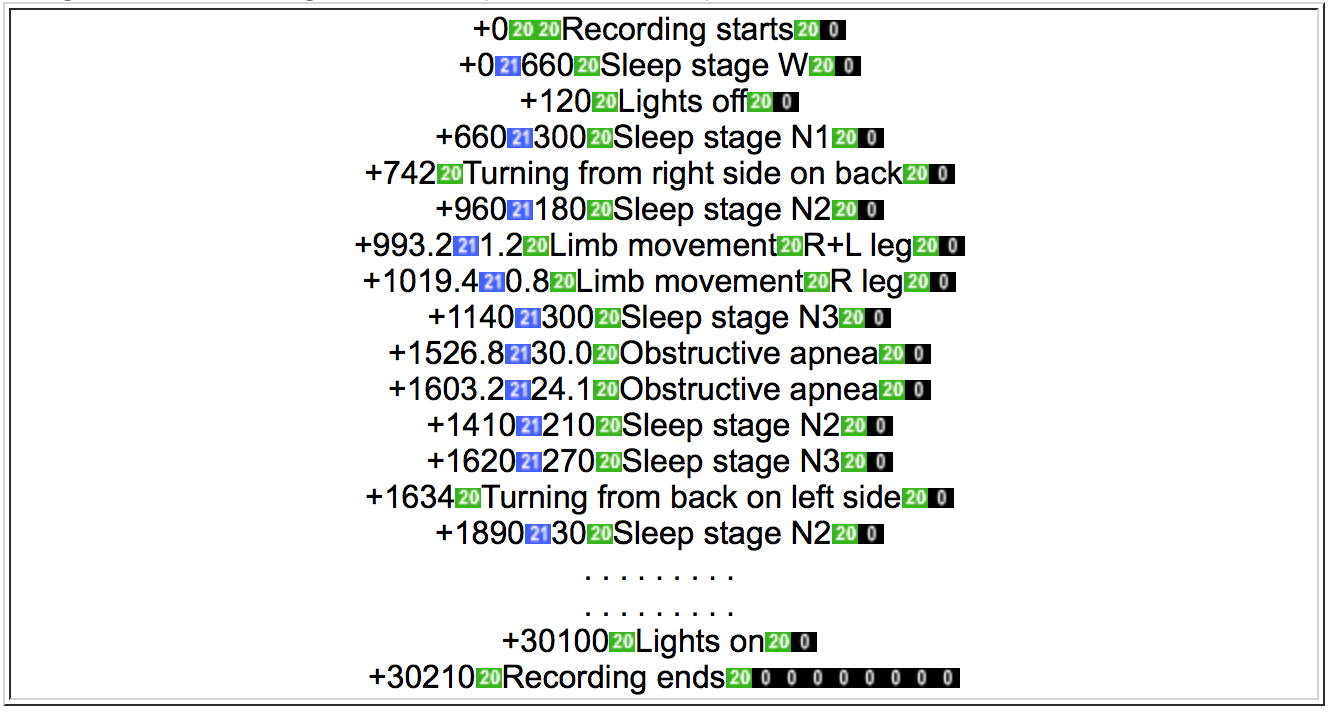
\includegraphics[width=1.0\textwidth]{Figures/Scoringsample.png}
            \caption{Sleep scoring sample\cite{EDFpluss}}
            \label{fig:Figures/Scoringsample}
        \end{figure}\\
        Figure 3.6 presents a sample of TALs for sleep scoring. The annotation signal is defined by giving it the label "EDF Annotations" in the label field in the header part. Then instead of storing ordinary signal samples, this field can be used for storing notation. This EDF annotations signal can be used for coding the text, time-keeping, events and stimuli as text. As presented in Figure 3.6, the annotations for sleep scoring are stored in TALs. Each TAL is formated in form +/-Onset21Duration20Annotation20Annotation20... Annotation20\textbf{0}, where 20, 21 and \textbf{0} are character codes. The Onset presents the amount of time before or after the starting time followed by a value 21 which is unprintable ASCII characters for ending the Onset. After the value 21 is the duration of this annotation. Both Onset and Duration can contains a dot character(float number) to make a better accuracy measurement. After the duration, each annotation can be separated by the unprintable ASCII character 20. The last annotation is followed by unprintable ASCII character 0 for terminating the list.\\
        In EDF+, the data records do not need to be contiguous. Therefore, the start time of each record must be specific. Although the first annotation of the first EDF annotations signal is empty, the timestamp of the annotation must be specified how many seconds after the recording started in term of date and time. Hence, the first TAL in the first data record must start with +0.X\textit{20}\textit{20}, X can be dropped if it is 0.
\section{CESAR data acquisition tools}
    First and foremost the sensor data which are generated by sensors need to be stored. Metadata needs to be defined such that the data can be easily sent, stored, and processed. This section presents two different tools that are used to obtain and store biosignals from different sensor sources (developed by Gjøby\cite{SP}), and from BITalino kit (developed by Carlos Carreiras et.al \cite{StorageBIT}).\\\\
    CESAR is a project that is under developed by a group of universities (University of Oslo, National University of Singapore and Oslo University Hospital). In the Master Thesis by Gjøby\cite{SP}, a generic data acquisition tool for mobile platforms (the Android platform) is presented. This tool is designed such that it is independent from data management and data analysis, and new data sources are also supported by it. An other tool which can be used to obtain biosignals for CESAR is StorageBIT. This tool was developed by Carlos Carreiras et.al \cite{StorageBIT}. StorageBIT is not only a data acquisition tool, but also a database model used for storing biosignals in an efficient way. Regarding the scope of this section, only data acquisition part of StorageBIT is presented in the section.
    \subsection{Generic Data Acquisition for Mobile Platforms}
    Gjøby finished his master degree with the project title "Generic Data Acquisition for Mobile Platforms" at the Department of Informatics at the University of Oslo in spring 2016. He worked on designing and developing an extensible system which allows applications to collect external and built-in sensor data through one common interface. He chose to design and implement a system for Android platform in his master thesis. He presents the overview of the system in the chapter "Not Android Specific". In this chapter, he explains how to design sensor wrappers and providers. A sensor wrapper establishes a connection to a specific data source in order to collect data, after that it sends the collected data to the provider application. Hence, the sensor wrapper needs to be designed to fit the technology of the link layer and communication protocol of the specific data source. Therefore, each data source has its own sensor wrapper. A provider is an extended sensor wrapper management which can use any of the available sensor wrappers. Figure 3.7 illustrates an overview of how sensor wrappers connect to a provider, and a way provider serves multiple applications.
    \begin{figure}[ht]
        \centering
        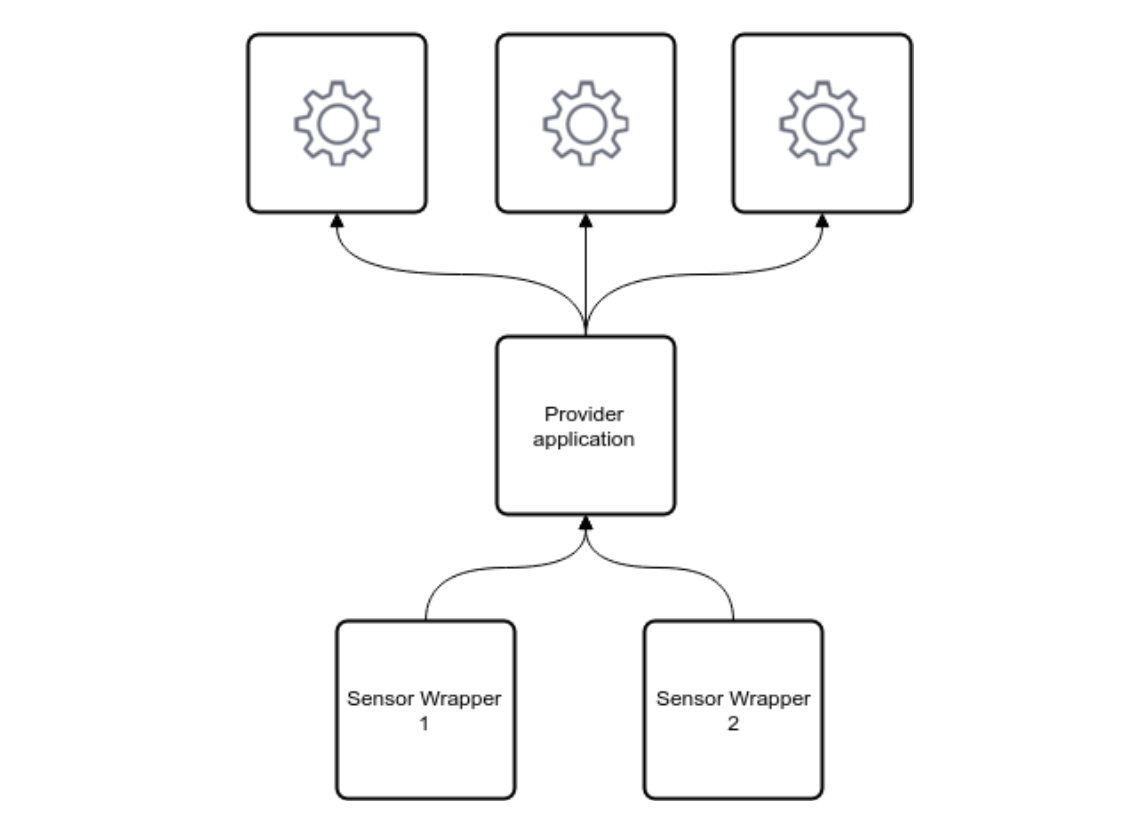
\includegraphics[width=0.5\textwidth]{Figures/provider_SW.png}
        \caption{Sharing the collected data between multiple applications\cite{SP}}
        \label{fig:provider_SW}
    \end{figure}\\
    In the chapter "Android Specific", he implements this design on the Android platform after discussing on the suitable components and functions that Android provides. To collect data from physical sensors and send the collected data to a user application, he defines two JSON structures as illustrates in the Figure 3.8. 
    \begin{figure}[ht]
        \centering     %%% not \center
        \subfigure[A JSON structure describing the encoding of the metadata]{\label{fig:stage}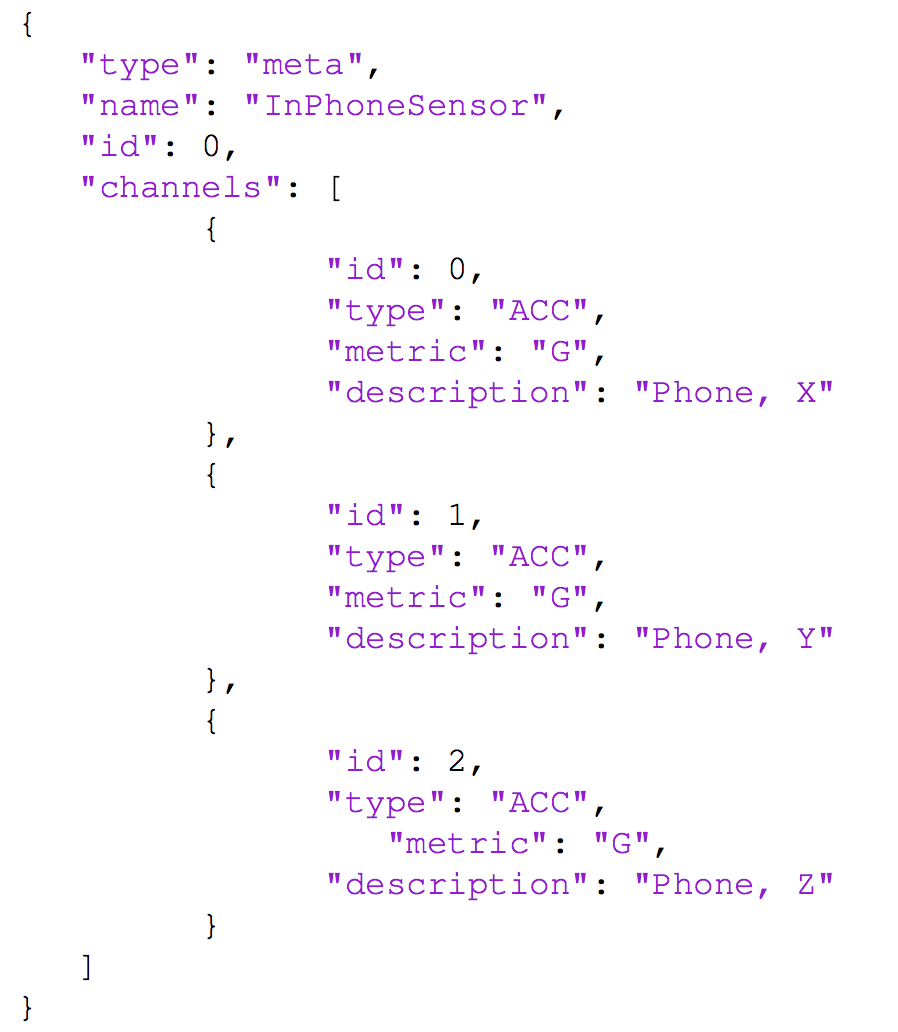
\includegraphics[width=70mm]{Figures/JSONmeta.png}}
        \subfigure[A JSON structure describing the encoding of a data reading]{\label{fig:respevt}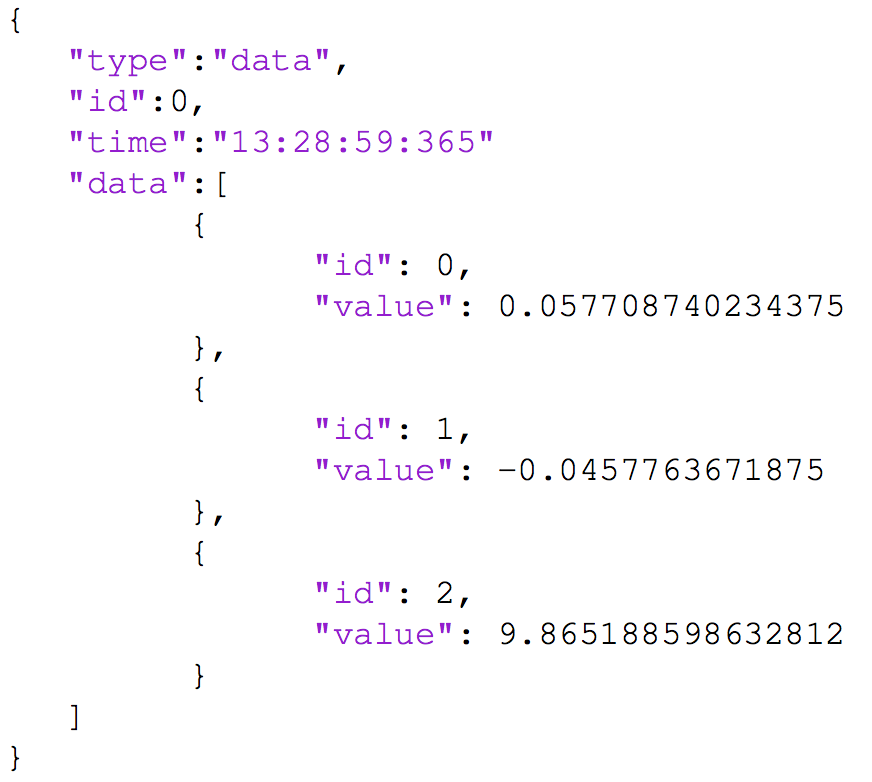
\includegraphics[width=75mm]{Figures/JSONdata.png}}
        \caption{A JSON structures used to send and receive sensor data.\cite{SP}}
        \end{figure}\\
    His application immediately sends a metadata to the application when it receives a connection demand. He defines the metadata in form of a JSON-Object which has as the first element a tuple("type","data"). The second and third elements are name and ID of the sensor wrapper, the remaining elements are the data from the channels, which belong to the sensor wrapper, in form of a JSON-Object array. Each channel has a unique id, type (ACC,ECG,EMG, etc.), metric and description. The JSON-Object is converted to a string and sent to the application. After connected to the BITalino board, the application retrieves data from physical sensors and submits to the application. The connection to the BITalino board should be stopped after receiving a stop signal from the application.\\
    As Gjøby presents in chapter "Not Android specific", the context of the data acquisition is specified as metadata for that it can be used for one common interface. After a comparison between JSON, XML and binary buffer, he decided to use JSON for streaming sensor data in his tool. At first, a metadata which contains general, unchanged information under acquisition (also known as a described context of the collected data from sensor wrapper) is sent, then the collected data from sensors are sent as soon as they are available to avoid overhead. The tool provides a common interface by combining the sensor wrapper ID and the channel ID as abstract level to identify each channel in the system. Figure 3.9 presents a sample of the metadata for BITalino by using a JSON structure. An existing sensor database can be treated as a sensor wrapper with a unique ID. The requested data for a channel in the sensor database can be obtained by using the database ID together with the ID of the requested channel. In other words, the metadata in form of JSON structure for all sensor sources are the same such that they can be used by a provider via one common interface.
    \begin{figure}[ht]
        \centering
        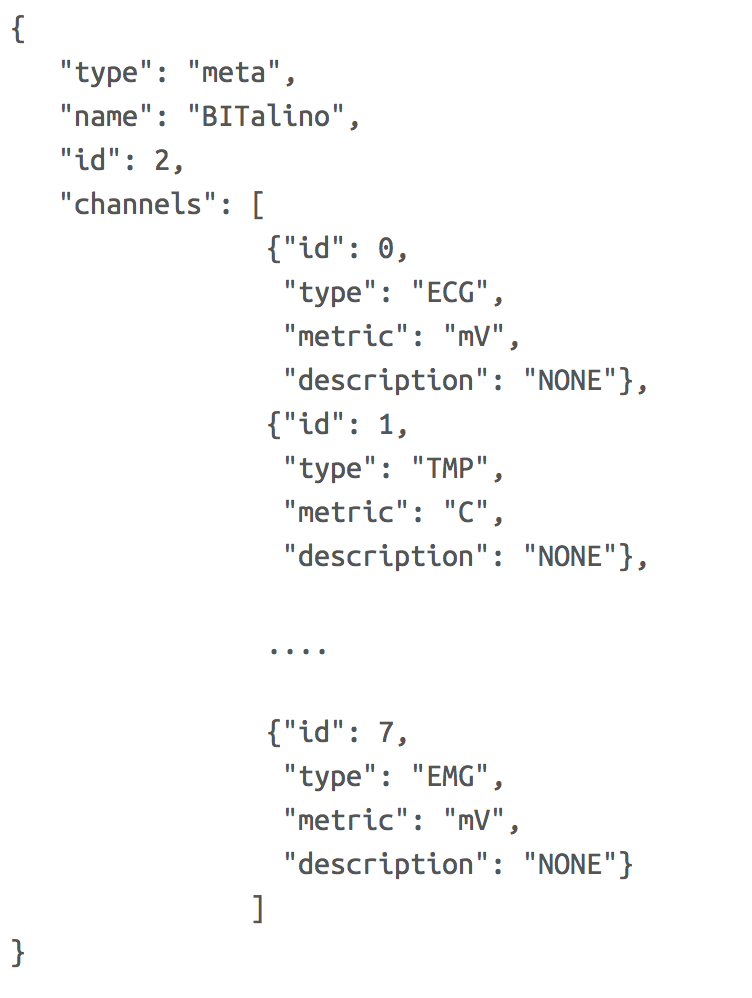
\includegraphics[width=0.5\textwidth]{Figures/metadata.png}
        \caption{A JSON structure sample of the metadata from BITalino}
        \label{fig:JsonGen}
    \end{figure}\\
    Each data sample contains type, sensor wrapper id, timestamp, and the data for the channels. The type of the sample must be "data" such that it can be distinguished with the metadata package which has the type "meta".\\
    Another important component in this tool is a provider. The provider can be considered as a bridge to connect the sensor wrappers with the applications. The provider works as a sensor wrapper management and data processing. It discovers sensor wrappers dynamically by broadcasting a discovery message, then it registers the responded sensor wrappers for later harvesting data. The collected data from sensor wrappers are pushed to the provider by using earlier mentioned JSON structure. Then, the provider processes the data, i.e, stores or forwards the data to an application.
    \subsection{StorageBIT data acquisition}
    Carlos Carreiras et.al \cite{StorageBIT} have done research on storing biosignals from BITalino. This tool can convert sensor data from different sources into their data model. Although the tool mainly supports the BITalino kit, it can also manage other sources by mirroring these sources into its data model. At first they make a comparison of the existing data formats which are the Extensible Biosignal File Format (EBS), the European Data Format (EDF and EDF+), the Medical Waveform Format Encoding Rules (MFER) and the Waveform Database(WFDB) based on eight properties which are compression, non-sequential access, cross platform support, events support, extensibility, metadata, multi modality and querying. After that, they make a data model which has "Records" as the basic abstract entities for storage. Each record consists of header, audit, biosignals and events and is stored in form of JSON-Object as presented in Figure 3.10. 
    \begin{figure}[ht]
        \centering
        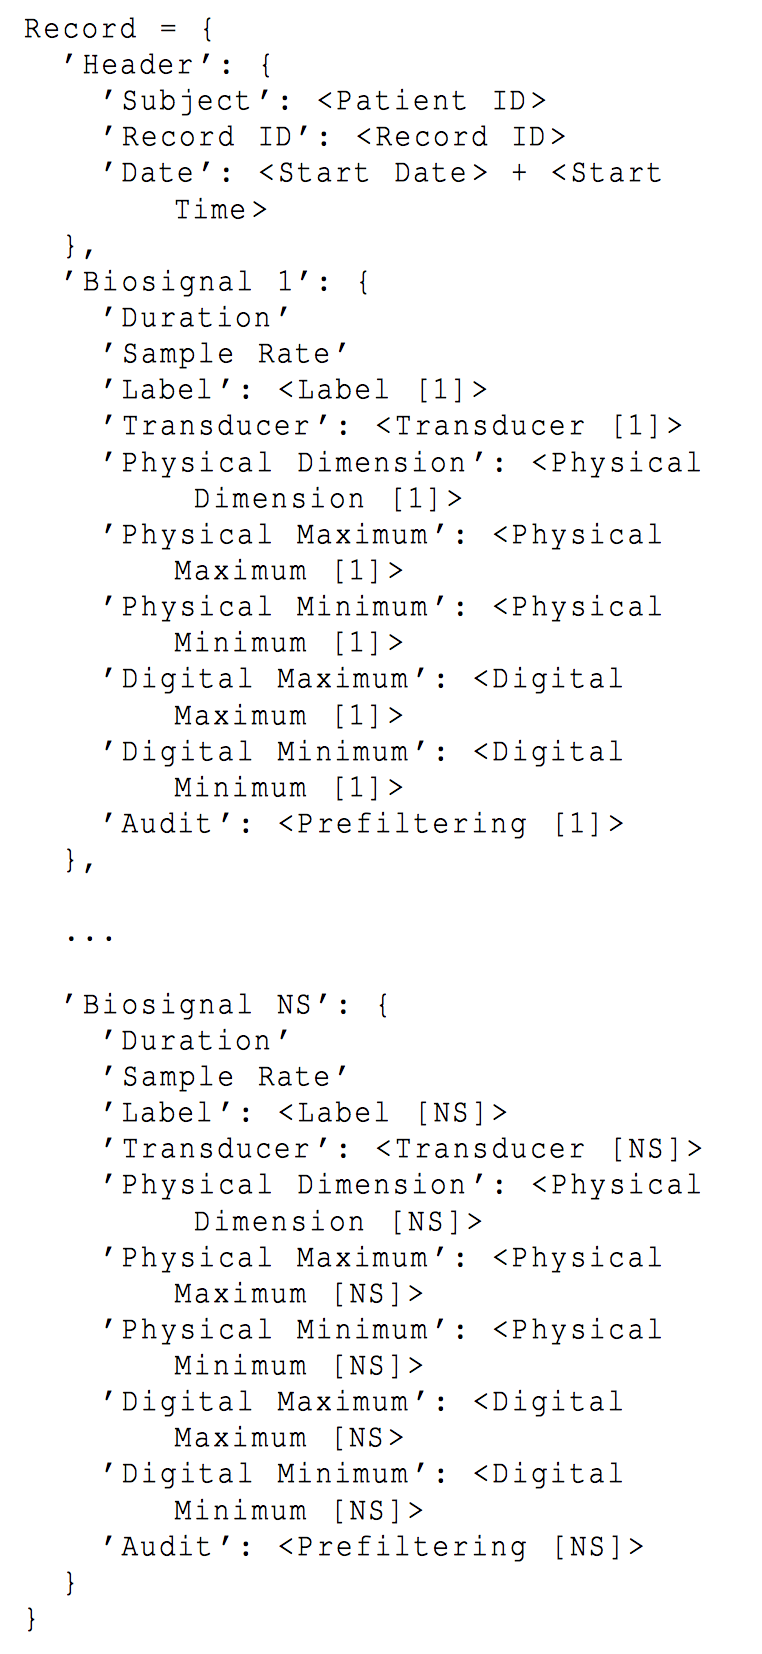
\includegraphics[width=0.5\textwidth]{Figures/metadata2.png}
        \caption{Mirroring of the EDF+ file structure onto the Data Model \cite{StorageBIT}}
        \label{fig:JsonStorageBIT}
    \end{figure}\\
    The header contains the basic information such as the patient identification, when and where the record was taken, and who performed the acquisition. The audit field contains the history of the file such as the applied filters or processing steps etc. The biosignal filed contains the data of the interested signals such as observing duration, sample rate, the label of the signal, transducer etc. The events field contains any asynchronized information like annotations or any events which are not synchronously from time series.